% !TeX root = ../thuthesis-example.tex
\chapter{相关工作}

\section{神经场表示}

与先前的三维网格、体素、点云的表示形式完全不同,神经场表示是三维几何表示方式的一个卓越革新,预示着三维内容生成和建模的范式转变。这一表示形式在2019年开始被发掘,并且很快成为热门。2021年发表的综述 Neural Fields in Visual Computing and Beyond \cite{neural_field_summary} 中对相关工作进行了总结整理,如图 \ref{fig:neural_field_pub} 所示,两年中已有近300篇工作使用了这一新兴表示。

\begin{figure}
  \centering
  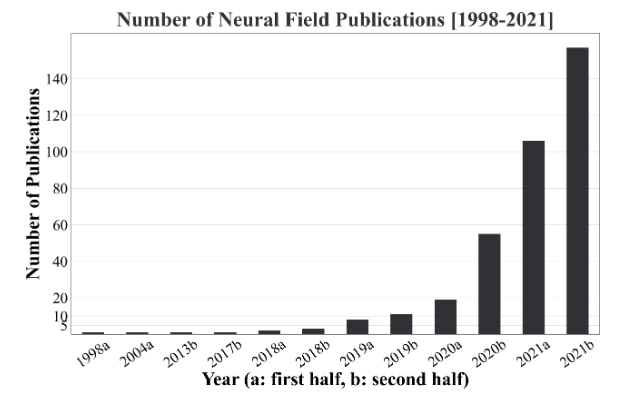
\includegraphics[width=0.9\linewidth]{neural_field_pub.png}
  \caption{神经场相关论文的发表情况}
  \label{fig:neural_field_pub}
\end{figure}

在视觉计算中,典型的神经场算法如下进行:在空间-时间范围内,我们对坐标进行采样,并将采样得到的坐标输入神经网络产生场量。场量的选取与我们的问题所需相对应。然后,我们用正向映射将场量重建为所需内容(例如RGB图像)。最后,我们通过重建信号与传感器收取到的真实信息(例如真实RGB图像)进行比较来计算重建误差和损失,从而引导神经网络的优化过程。

在一系列相关工作中,神经辐射场(NeRF)\cite{nerf} 是最具代表性的方法之一。他成功地将神经场表示引入到三维重建问题中,并且取得了很好的效果,并被广泛应用于新视角合成等问题,沿用至今。因此接下来我们将对其展开介绍。

\subsection{神经辐射场(NeRF)}

神经辐射场的核心在于其场量表示。如下所示:
\begin{equation}
  F(\mathbf{x},\mathbf{d})\to(\mathbf{c},\sigma),
\end{equation}

其中 $\mathbf{x}=(x,y,z)$ 代表三维空间中的坐标,$\mathbf{d}$ 表示视角。输出部分的 $\mathbf{c} = (r,g,b)$ 表示颜色,$\sigma$ 表示密度。$F$ 通常用多层感知机(MLP)来近似。值得注意的是,$\sigma$ 仅是关于 $\mathbf{x}$ 的函数,以此来保证多视角下的一致性,而颜色 $\mathbf{c}$ 同时依赖于位置 $\mathbf{x}$ 和视角 $\mathbf{d}$。

重建过程采用体渲染。在实际物理过程中,光线从光源出发,经过物体表面反射后到达相机。由于光路可逆,我们可以假定从相机处射出光线。对于每一条从相机处发出的光线,我们通过均匀采样或其他采样方法,生成一组采样点,并根据体渲染的渲染公式计算出像素对应的颜色。设相机光线 $\mathbf{r}(t)=\mathbf{o}+t\mathbf{d}$,其中 $\mathbf{o}$表示相机位置,$\mathbf{d}$表示光线方向,则该像素对应的颜色按照下式计算:
\begin{equation}
  C(\mathbf{r})=\int_{t_n}^{t_f}T(t)\sigma(\mathbf{r}(t))\mathbf{c}(\mathbf{r}(t),\mathbf{d}) \mathrm{d}t , \ \mathrm{where} \ \ T(t)=\exp\left(-\int_{t_n}^t\sigma(\mathbf{r}(s))ds\right).
\end{equation}

我们通过采样来估计这个积分。以均匀采样为例,我们在区间 $[t_n,t_f]$ 上采样 $N$ 个点:
\begin{equation}
  t_i\sim\mathcal{U}\bigg[t_n+\frac{i-1}{N}(t_f-t_n), t_n+\frac{i}{N}(t_f-t_n)\bigg],
\end{equation}
并用这些样本来估计 $C(\mathbf{r})$:
\begin{equation}
  \hat C(\mathbf{r})=\sum_{i=1}^NT_i(1-\exp(-\sigma_i\delta_i))\mathbf{c}_i , \ \mathrm{where} \ \ T_i=\exp\left(-\sum_{j=1}^{i-1}\sigma_j\delta_j\right).
\end{equation}

虽然许多神经场表示方法将三维几何形状表示为如上的密度场,但近期有符号距离场(SDF)也开始被广泛使用。有符号距离场可以方便地表示几何形状的边界,因此可以导出三维网格表示,这是密度场所无法做到的。然而,这一转化也导致了渲染质量的显著降低。我们的工作通过将密度场转化为SDF场,再将SDF场转化为高质量连续曲面网格,并通过可微渲染保证了渲染质量。这种转换不仅确保了出色的渲染质量,还拓展了后续下游应用的范围。此外,导出三维网格表示与相应的材料、纹理和光照,使其不再借助神经场表示和神经网络,而是可以直接应用在渲染器中,加速了渲染速度。

\section{可微渲染}

如前所述,渲染是从三维场景得到二维图像的过程。可微渲染则是指这一过程是可微的,即我们可以计算渲染结果对输入场景的梯度,其中输入场景一般包括几何、材质和光照等信息。可微渲染在计算机图形学和计算机视觉中有着广泛的应用,例如图像生成、三维重建、逆渲染等问题。传统渲染管线一般并不可微,主要原因是光线与物体表面的交互是不可导的。因此,可微渲染的一般思路一般是在传统渲染管线中引入可微的近似方法,或者更改渲染算法的某些部分使其可微。本文主要涉及到可微光栅化和可微光线追踪,因此下面对这两个方向的相关工作进行介绍。

\subsection{可微光栅化}

可微光栅化是可微渲染中的重要方法,相关的研究也相对深入。它在传统渲染技术和现代深度学习之间搭建了新的桥梁。可微属性使得网络能够直接从图像数据中学习并优化几何属性,从而端到端地完成三维重建和逆渲染任务。可微光栅化主要目的在于提升性能,它们以局部光照为前提,着色时仅考虑局部阴影,重点在于强调获得有用的可见性梯度,以通过梯度下降优化几何形状。

Shichen Liu 等人提出了 Soft Rasterizer \cite{softraster}。这个工作将确定性的渲染过程看做一个”软“的概率过程。传统的光栅化过程中,对于每个像素,仅选择最上层的三角形片元进行着色。而在 Soft Rasterizer 中,我们将每一个三角形都视作概率云,每一层的三角形都对最终颜色有一定概率贡献。他们提出了一种可微聚合函数,根据概率图和三角形的相对深度融合每个三角形的颜色图,形成最终的渲染结果。这种新的渲染方法使得他们可以将梯度回传到每一层三角形上,包括在传统光栅化意义下被遮挡的三角形。

Soft Rasterizer通过修改传统渲染方法使其变得可微。与之不同,OpenDR \cite{OpenDR} 并没有对前向渲染算法做出任何修改,而是通过在反向传播过程中近似计算梯度来解决该问题。它将像素分为内部像素、边界像素和多边界像素三类分别进行处理,并将图像颜色的梯度近似为像素颜色的差分。

Nvdiffrast \cite{nvdiffrast} 的目标同样是在不更改传统渲染方法的情况下实现可微光栅化。因此在他们的设定下,对于最终图像没有产生影响的片元,例如由于遮挡或者超出屏幕外的部分,梯度应当为零。他们实现了模块化的框架,主要包含光栅化、插值、纹理过滤和抗锯齿四个部分,通过抗锯齿将边界处的不连续性平滑化,从而可以计算梯度。本文中可微光栅化的部分主要借助 Nvdiffrast 实现。

\subsection{可微光线追踪}

相较于可微光栅化,可微光线追踪相关的研究相对较少。这是因为光线追踪的计算复杂度较高,逆渲染时一般不会考虑光线追踪,而且光线追踪的过程中由于存在很多不可导的操作。由于光线追踪需要光线的多次反射,几何形状的微小改变可能会改变每一次反射的方向,叠加起来就会对整条光路产生巨大的影响。与可微光栅化类似,可微光线追踪的主要思路也是通过近似让计算关于几何形状的梯度成为可能。在这个过程中,我们需要考虑到光线追踪的复杂性,以及如何在保证计算效率的同时保证梯度的准确性。

Tzu-mao Li 等人提出的 redner \cite{DiffMCRT} 将渲染的计算分成平滑区域和不连续区域。对于平滑区域,他们采用传统的面积采样方式,并通过边采样替代面积采样的方式解决边界处场景函数关于参数不可导的问题。

Loubet 等人提出了一种重参数化积分的方式来处理不连续问题 \cite{Loubet}。一般来说,光线追踪需要计算如下积分式:
\begin{equation}
  I=\int_{\mathcal X}f(x,\theta) \mathrm{d}x,
\end{equation}
其中积分区域 $\mathcal X$ 通常是球面。所谓的不可导问题是指 $f(x, \theta)$ 由于边界处可见性的变化关于场景参数 $\theta$ 不可导。Loubet 等人通过在 $\theta$ 的邻域 $U(\theta)$ 内找到一个变换 $T: U(\theta)\times\mathcal Y\to\mathcal X$,使得 $T$ 是可导的,从而将积分转化为:
\begin{equation}
  \int_{\mathcal{X}}f(x,\theta) \mathrm{d}x=\int_{\mathcal{Y}}f(T(y,\theta),\theta) |\det J_T| \mathrm{d}y.
\end{equation}
在这种变换后,采样过程中不连续的位置不再随场景参数变化而变化。这也就解决了不可导问题。

Zhang 等人先后提出了 PhySG \cite{PhySG} 和 IRON \cite{IRON} 两个可微渲染框架。PhySG 仅仅考虑直接光照,并不考虑自遮挡和简介光照。他们用球形高斯对环境光进行建模,用 SDF场表示几何形状,并通过法向量的梯度回传至SDF场上来优化几何表示。IRON 则是PhySG 后的进一步工作,他们继承了PhySG 的 SDF场表示,并通过类似于 redner 的基于边缘感知物理的表面渲染优化各个参数。

在另一个名为 Path-space differentiable rendering \cite{PSDR} 的工作中,作者通过复杂的数学推导,直接在路径空间中考虑路径的微分。他们将路径积分的微分分解为内部项和边界项两部分,并在路径空间中分别使用蒙特卡洛方法进行估计。对于边界项,他们采用了一种完全可微的采样方法,因此其导数计算可以非常精确。但这种方法对单个渲染图像的梯度计算需要数十秒的时间,因而不适合于神经网络的训练。


\section{逆渲染}

如前所述,逆渲染旨在从一张或一组图像中获取对场景的物理属性的理解,包括三维几何信息、材质、光照、纹理等等。由于该问题不适定,大部分逆渲染相关的工作都对光照、形状做出一些假设,甚至给定光照条件,或是结合关于光照、阴影、材质、几何形状等的先验知识。

早期的工作借助大量先验来简化问题。Barron 等人在2015年提出的工作中\cite{SIRS},根据形状、反射率和照明的一组先验,将问题表述为统计推理和优化之一。他们将问题规约成:
\begin{equation*}
  \begin{array}{ccc}\text{maximize}_{R,Z,L}&&P(R)P(Z)P(L)\\\text{subject to}&&I=R+S(Z,L)\end{array}.
\end{equation*}
其中,$R$ 是对数反射图像,$Z$ 是深度图,$L$ 是用球谐函数表示的光照。$S(Z,L)$是一个渲染引擎。$P(R), P(Z), P(L)$ 分别是反射率、形状和光照的先验。他们希望重建的模型尽量符合先验,同时需要符合输入图像。由于使用了大量先验,在此不做赘述,我们仅以形状为例,作者希望重建的形状符合以下几个条件:
\begin{itemize}
  \item 光滑。通过最小化曲率的变化来实现。
  \item 表面法线各向同性。我们希望邻近点的法线方向尽量一致。
  \item 边缘处法线约束。理想情况下,假设相机从垂直方向拍摄,则物体边缘处法线应该与边缘垂直,$z$ 分量为零。
\end{itemize}
通过将这些假设数学化,加入到优化问题中,作者最终得到了一个能够重建物体形状、反射率和光照的优化算法。

与上述工作不同,Zhengqin Li 等人通过建立一个大规模形状材质数据集来获取关于形状和材质的先验,并且提出了新的网络架构整体上解决逆渲染问题 \cite{Learning1image}。通过大规模数据集,他们用不同的方式获取了非常强的先验,从而能从单张图片还原出物体的三维形状和材质。

在计算机视觉中,还有部分工作通过估计深度图来还原三维形状。在 Deep 3D Capture \cite{D3DC} 中,输入的多张图像首先经过深度估计网络得到深度图,根据深度图完成图像的粗对齐。接着,通过编码-解码网络,从图像中提取材质、法线等信息,并且通过估计的深度图结合这些信息得到图像,并与真实图像对比来优化网络。这种方法对深度估计的准确性要求较高,且对于复杂的场景,往往难以得到满意的结果。

还有部分工作专注于简单的材质模型。Chen 等人在2021年的工作中,针对没有纹理的简单物体设计了新颖的逆渲染框架。他们在合成数据和真是图像上都获得了相当精细出色的结果。但除了材质模型的假设之外,他们还有一些其他约束,例如光照和相机的绑定、仅使用点光源等。这也就导致这个工作的应用范围受到限制。

\section{小结}

本章介绍了神经场表示、可微渲染和逆渲染等相关工作。神经场表示作为三维几何表示的一种革新,引领了三维内容生成和建模的新方向。可微渲染在传统渲染技术和深度学习方法之间搭建了桥梁,使得渲染过程可导,有助于端到端的三维重建和逆渲染任务。逆渲染则旨在从图像中推断出场景的物理属性,但可以看到,由于逆渲染问题自身的不适定性,多数方法都做了较强的先验和假设。可微渲染也是逆渲染的重要方法之一,可微光栅化常常作为逆渲染中的重要模块,但可微光线追踪由于计算复杂度较高,较少被应用于逆渲染问题。
目前看来,三维重建和逆渲染还不存在一个通用的解决方案。通过神经辐射场,我们可以得到高质量的视觉效果,但其密度场表示并不适合后续应用。而逆渲染方法同样局限,即使能够得到物体表面的反射率、粗糙度等信息,也无法避免会将照明伪影等信息“烘焙”到材质中。如何将可微光线追踪应用于逆渲染问题,是一个值得深入挖掘的方向。
